% (c) 2002 Matthew Boedicker <mboedick@mboedick.org> (original author) http://mboedick.org
% (c) 2003-2007 David J. Grant <davidgrant-at-gmail.com> http://www.davidgrant.ca
% (c) 2008 Nathaniel Johnston <nathaniel@nathanieljohnston.com> http://www.nathanieljohnston.com
% (c) 2011 Scott Clark <sc932@cornell.edu> http://cam.cornell.edu/~sc932
% (c) 2012 Arne Hassel <arne.hassel@gmail.com> http://megoth.wordpress.com/
%
%This work is licensed under the Creative Commons Attribution-Noncommercial-Share Alike 2.5 License. To view a copy of this license, visit http://creativecommons.org/licenses/by-nc-sa/2.5/ or send a letter to Creative Commons, 543 Howard Street, 5th Floor, San Francisco, California, 94105, USA.

\documentclass[letterpaper,11pt,norsk]{article}
\newlength{\outerbordwidth}
\pagestyle{empty}
\raggedbottom
\raggedright
\usepackage{array}
\usepackage{babel}
\usepackage{colortbl}
\usepackage{color}
\usepackage{float}
\usepackage[T1]{fontenc}
\usepackage{framed}
\usepackage{graphicx}
\usepackage{ifthen}
\usepackage[utf8]{inputenc}
\usepackage{tocloft}
\usepackage{url}
\usepackage[svgnames]{xcolor}
\usepackage{wrapfig}

%-----------------------------------------------------------

%Edit these values as you see fit

\setlength{\outerbordwidth}{3pt}  % Width of border outside of title bars
\definecolor{shadecolor}{gray}{0.75}  % Outer background color of title bars (0 = black, 1 = white)
\definecolor{shadecolorB}{gray}{0.93}  % Inner background color of title bars

%-----------------------------------------------------------

%Margin setup

\newlength{\cellwidth}
\newlength{\colmainwidth}
\newlength{\tablewidth}

\setlength{\cellwidth}{0.2in}
\setlength{\colmainwidth}{3.4in}
\setlength{\evensidemargin}{-0.25in}
\setlength{\headheight}{-0.25in}
\setlength{\headsep}{0in}
\setlength{\oddsidemargin}{-0.25in}
\setlength{\paperheight}{11in}
\setlength{\paperwidth}{8.5in}
\setlength{\tablewidth}{7in}
\setlength{\tabcolsep}{0in}
\setlength{\textheight}{9.75in}
\setlength{\textwidth}{7in}
\setlength{\topmargin}{-0.3in}
\setlength{\topskip}{0in}
\setlength{\voffset}{0.1in}

%-----------------------------------------------------------

%Custom commands

\newcommand{\resitem}[1]{\item #1 \vspace{-2pt}}

\newcommand{\resheading}[1]{\vspace{8pt}
  \parbox{\textwidth}{\setlength{\FrameSep}{\outerbordwidth}
    \begin{shaded}
\setlength{\fboxsep}{0pt}\framebox[\textwidth][l]{\setlength{\fboxsep}{4pt}\fcolorbox{shadecolorB}{shadecolorB}{\textbf{\sffamily{\mbox{~}\makebox[6.762in][l]{\large #1} \vphantom{p\^{E}}}}}}
    \end{shaded}
  }\vspace{-5pt}
}

\newcommand{\ressubheading}[4]{
\begin{tabular*}{6.5in}{l@{\cftdotfill{\cftsecdotsep}\extracolsep{\fill}}r}
		\textbf{#1} & #2 \\
		\textit{#3} & \textit{#4} \\
\end{tabular*}\vspace{-6pt}}

\newcommand{\forloop}[6][1]%
{%
\setcounter{#2}{#3}%
\ifthenelse{#4}%
	{%
	#6%
	\ifthenelse{#5}{\arabic{#2}}{\hspace{3mm}}
	\addtocounter{#2}{#1}%
	\forloop[#1]{#2}{\value{#2}}{#4}{#5}{#6}%
	}%
% Else
	{%
	}%
}%

\newcounter{ct}
\newcounter{kl}
\newcounter{klm}
\newcounter{wl}
\newcounter{wlm}
\newcommand{\skill}[3]{
	\setcounter{ct}{-1}
	\setcounter{kl}{#2}
	\setcounter{klm}{#2}
	\setcounter{wl}{#3}
	\setcounter{wlm}{#3}
	
	\addtocounter{klm}{1}
	\addtocounter{wlm}{1}
	
	#1
	\forloop{ct}{1}{\value{ct} < \value{klm}}{\value{ct} = \value{kl}}%
	{%
	& \cellcolor[gray]{0.5}
	}
	\forloop{ct}{\value{klm}}{\value{ct} < \value{wlm}}{\value{ct} = \value{wl}}%
	{%
	& \cellcolor[gray]{0.9}
	}
	\forloop{ct}{\value{wlm}}{\value{ct} < 11}{\value{ct} = 11}%
	{%
	& \cellcolor[gray]{1}
	}
	\\
}

\newcommand{\skilltable}[2]{
	\vspace{2.5mm}
	\begin{tabular}{p{1.5in} l*{10}{c}}
		\textbf{\Large #1} & 1 & 2 & 3 & 4 & 5 & 6 & 7 & 8 & 9 & 10 \\
		\hline
		#2
	\end{tabular}
}

%-----------------------------------------------------------

\title{Curriculum Vitae}

\begin{document}

\begin{minipage}{\textwidth}
\begin{wrapfigure}{r}{0pt}
	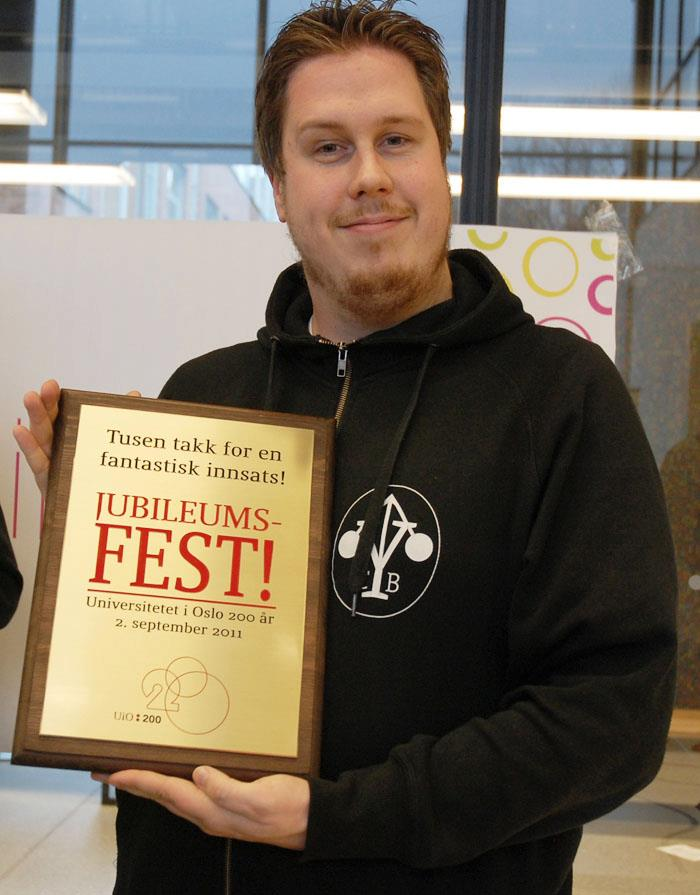
\includegraphics[height=45mm]{uio200.jpg}
\end{wrapfigure}

\textbf{\Large Kompetansediagram for Arne Hassel}

\vspace{5mm}

\begin{minipage}{5in}

Kompetansediagrammene gir en oversikt over min kompetanse både faglig, personlig og sosialt. Det er en videreføring av CVen og gir en bedre oversikt innen de ulike kompetanseområdene. Diagrammene er selvkritiske og personlige, og det er benyttet en skala fra 0 til 10 for å vektlegge hvor god kompetanse jeg har innen de forskjellige områdene. 0, ingen skravering, betyr ingen kompetanse og 10, full skravering, betyr maks kompetanse innen et felt. Områder jeg har særdeles interesse innen og ønsker å forbedre meg i har jeg uttrykt ved å skravere i en lysere nyanse til det nivået jeg ønsker å nå.
\end{minipage}

\end{minipage}

\resheading{Informatikk}

\begin{tabular*}{\tablewidth}{p{\colmainwidth}@{\extracolsep{\fill}}p{\colmainwidth}}
\skilltable{Teori}{%
	\skill{Algoritmer}{4}{7}
	\skill{Databaser}{7}{9}
	\skill{Datamaskinarkitektur}{3}{5}
	\skill{Datastrukturer}{6}{7}
	\skill{Design patterns}{7}{9}
	\skill{Kvalitativ forskning}{6}{7}
	\skill{Logikk}{4}{8}
	\skill{Matematikk}{5}{8}
	\skill{Modellering}{7}{8}
	\skill{Semantiske teknologier}{7}{9}
	\skill{Statistikk}{3}{6}
	\skill{Systemutvikling}{7}{10}
}%
&
\skilltable{Programmering}{%
	\skill{Assembly}{2}{2}
	\skill{C}{4}{6}
	\skill{C\#}{5}{8}
	\skill{Dokumentasjon}{5}{9}
	\skill{Java}{5}{6}
	\skill{JavaScript}{5}{10}
	\skill{PHP}{4}{6}
	\skill{Python}{4}{9}
	\skill{Regex}{3}{9}
	\skill{SPARQL}{4}{7}
	\skill{SQL}{6}{7}
	\skill{Testing (TDD)}{5}{9}
	\skill{XSLT}{5}{5}
}%
\\
\skilltable{Stilark språk}{%
	\skill{CSS}{8}{10}
	\skill{LESS}{6}{8}
	\skill{Sass}{5}{8}
}% 
&
\skilltable{Markup}{%
	\skill{HTML}{8}{10}
	\skill{Turtle}{8}{9}
	\skill{XML}{5}{5}
}% 
\\
\skilltable{Design}{%
	\skill{Design for mobil}{5}{9}
	\skill{Grafisk design}{3}{5}
	\skill{Informasjonsdesign}{4}{9}
	\skill{Interaksjonsdesign}{5}{8}
	\skill{Responsive design}{7}{10}
}% 
&
\skilltable{Rammeverk}{%
	\skill{Compass}{6}{9}
	\skill{Django}{3}{8}
	\skill{jQuery}{7}{10}
	\skill{.NET MVC 2}{4}{5}
	\skill{.NET MVC 3}{3}{8}
	\skill{Umbraco}{5}{5}
	\skill{Wordpress}{4}{6}
}% 
\\
\skilltable{Operativsystem}{%
	\skill{OSX}{6}{7}
	\skill{Ubuntu}{4}{9}
	\skill{Windows 7}{8}{8}
	\skill{Windows Vista}{7}{7}
	\skill{Windows XP}{8}{8}
}%
&
\skilltable{Programpakker}{%
	\skill{MS Office}{8}{8}
	\skill{Open Office}{6}{7}
	\skill{Photoshop CS4}{4}{6}
	\skill{Visual Studio}{7}{9}
}% 
\end{tabular*}

\resheading{Personlig}

\begin{tabular*}{\tablewidth}{p{\colmainwidth}@{\extracolsep{\fill}}p{\colmainwidth}}
\skilltable{Egenskaper}{%
	\skill{Analytisk}{6}{8}
	\skill{Ansvarsbevist}{7}{7}
	\skill{Avbalansert}{7}{7}
	\skill{Effektiv}{7}{8}
	\skill{Fornuftig}{7}{7}
	\skill{Kreativ}{6}{8}
	\skill{Lojal}{9}{9}
	\skill{Nysgjerrig}{8}{8}
	\skill{Positiv holdning}{7}{7}
	\skill{Samvittighetsfull}{7}{7}
	\skill{Selvstendig}{8}{8}
	\skill{Strukturert}{7}{8}
}%
&
\skilltable{Evne til å:}{%
	\skill{Gi kritikk}{6}{8}
	\skill{Gi ros}{5}{8}
	\skill{Lytte}{5}{8}
	\skill{Motivere andre}{7}{7}
	\skill{Samarbeide}{7}{8}
	\skill{Si nei}{8}{8}
	\skill{Takle motgang}{7}{8}
	\skill{Tilegne kunnskap}{7}{10}
}%
\\
\skilltable{Sosial}{%
	\skill{Imøtekommende}{7}{7}
	\skill{Inkluderende}{8}{8}
	\skill{Omgjengelig}{6}{6}
	\skill{Serviceinnstilt}{7}{7}
	\skill{Utadvent}{6}{6}
}%
\end{tabular*}

\resheading{Annet}

\begin{tabular*}{\tablewidth}{p{\colmainwidth}@{\extracolsep{\fill}}p{\colmainwidth}}
\skilltable{Administrasjon}{%
	\skill{Ledelse}{5}{9}
	\skill{Organisasjonsanalyse}{3}{7}
	\skill{Risikoanalyse}{3}{7}
	\skill{SWOT-analyse}{3}{5}
}%
&
\skilltable{Økonomi}{%
	\skill{Bilagsføring}{7}{7}
	\skill{Budsjett}{6}{7}
	\skill{Regnskap}{7}{7}
	\skill{Samfunnsøkonomi}{5}{5}
}%
\\
\skilltable{Språk}{%
	\skill{Norsk}{9}{10}
	\skill{Engelsk}{8}{10}
	\skill{Tysk}{2}{2}
}%
\\
\end{tabular*}

\end{document}
